\section{DevOps: Infraestrutura}

\subsection{Introdução}

A infraestrutura de rede apresentada foi desenvolvida para atender às necessidades de comunicação e gerenciamento da plataforma de verificação do teste do iodo por visão computacional aplicada à produção de cerveja artesanal.

A rede é responsável por interligar servidor, computador de monitoramento, dispositivos móveis e equipamentos de comunicação, garantindo estabilidade na transmissão dos dados, armazenamento das análises e acesso à aplicação web. Além disso, a infraestrutura permite comunicação entre os componentes do sistema utilizados durante o processo de mosturação.

\subsection{Topologia da Rede}

A infraestrutura utiliza topologia em estrela, na qual todos os dispositivos estão conectados a um switch central localizado na sala técnica. O switch está ligado ao modem/roteador responsável pelo acesso à internet e funcionamento como gateway padrão da rede. Essa abordagem facilita a manutenção, gerenciamento e expansão futura da infraestrutura.

\subsection{Estrutura da Rede}

A rede cabeada utiliza cabos Ethernet padrão Cat6, proporcionando maior estabilidade e velocidade na transmissão dos dados. O servidor possui endereço IP fixo e é responsável pelo armazenamento e gerenciamento das informações do sistema.

Além da rede cabeada, a infraestrutura também possui suporte à comunicação sem fio por meio de um ponto de acesso Wi-Fi instalado na sala técnica, permitindo conexão de dispositivos móveis utilizados durante o processo de produção e monitoramento da plataforma.

\begin{table}[H]
\centering
\caption{Endereçamento da Rede}
\label{tab:rede}
\begin{tabular}{|l|l|p{6cm}|}
\hline
\textbf{Dispositivo} & \textbf{Endereço IP} & \textbf{Observação} \\
\hline
Roteador / Gateway & 192.168.0.1 & Acesso à internet \\
\hline
Servidor & 192.168.0.2 & Armazenamento de dados \\
\hline
Computador da Sala Técnica & 192.168.0.10 & Monitoramento do sistema \\
\hline
Dispositivos móveis & DHCP automático & Conexão Wi-Fi \\
\hline
\end{tabular}
\end{table}

\subsection{Arquitetura de Rede}

\begin{table}[H]
\centering
\caption{Componentes da Infraestrutura da Rede}
\label{tab:infraestrutura}
\begin{tabular}{|l|p{10cm}|}
\hline
\textbf{Componente} & \textbf{Descrição} \\
\hline

\textbf{Roteador / Gateway} &
\begin{itemize}[leftmargin=*, nosep]
    \item Responsável pelo acesso à internet
    \item Atua como gateway padrão da rede
    \item Distribuição da comunicação da rede local
\end{itemize} \\
\hline

\textbf{Switch Central} &
\begin{itemize}[leftmargin=*, nosep]
    \item Interligação dos dispositivos da rede
    \item Estrutura central da topologia estrela
    \item Facilita expansão e manutenção da infraestrutura
\end{itemize} \\
\hline

\textbf{Servidor} &
\begin{itemize}[leftmargin=*, nosep]
    \item Processamento das análises do sistema
    \item Execução da aplicação Flask
    \item Armazenamento dos dados e resultados
\end{itemize} \\
\hline

\textbf{Computador da Sala Técnica} &
\begin{itemize}[leftmargin=*, nosep]
    \item Monitoramento do sistema
    \item Gerenciamento operacional da plataforma
    \item Controle local da aplicação
\end{itemize} \\
\hline

\textbf{Dispositivos Móveis} &
\begin{itemize}[leftmargin=*, nosep]
    \item Captura das imagens do teste do iodo
    \item Acesso remoto à plataforma
    \item Comunicação via rede Wi-Fi
\end{itemize} \\
\hline

\end{tabular}
\end{table}

\subsection{Diagrama de Infraestrutura}

A Figura \ref{fig:diagrama-de-infraestrutura} apresenta o diagrama da infraestrutura utilizada na plataforma, demonstrando a comunicação entre os dispositivos da rede.

\begin{figure}[H]
\centering
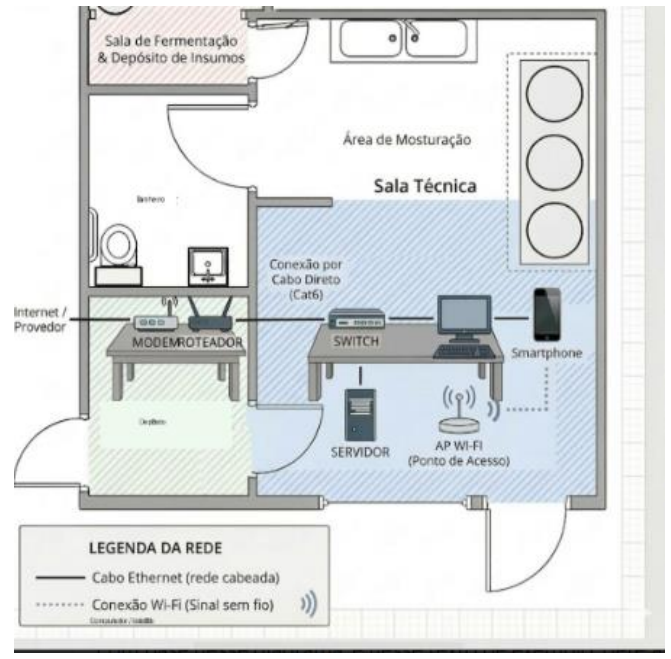
\includegraphics[width=0.9\linewidth]{imgs/redes.png}
\caption{Diagrama de Infraestrutura do Sistema}
\label{fig:diagrama-de-infraestrutura}
\end{figure}

\subsection{Diagrama de Usabilidade}

A Figura \ref{fig:diagrama-de-usabilidade} apresenta o diagrama de usabilidade da plataforma, demonstrando o fluxo de interação entre o funcionário e os principais componentes do sistema. O diagrama evidencia como o usuário acessa a aplicação, envia a imagem do teste do iodo, recebe o resultado da análise e consulta as informações armazenadas.

\begin{figure}[H]
\centering
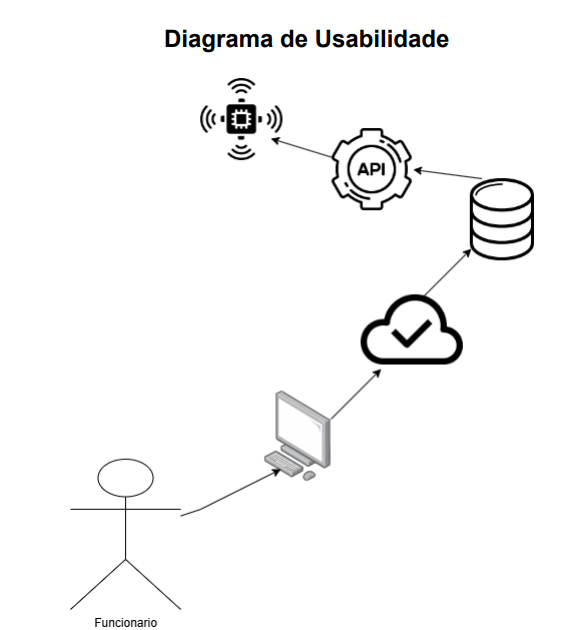
\includegraphics[width=0.9\linewidth]{imgs/usabilidade.png}
\caption{Diagrama de Usabilidade}
\label{fig:diagrama-de-usabilidade}
\end{figure}

\subsection{Conclusão}

A infraestrutura proposta oferece uma solução simples, funcional e segura para o ambiente de produção da cervejaria artesanal. A utilização da topologia em estrela facilita o gerenciamento da rede, melhora a comunicação entre os dispositivos e permite futuras expansões do sistema, incluindo integração com novas soluções de automação e monitoramento.